\documentclass[12pt]{article}
\usepackage[utf8]{inputenc}
\usepackage[english]{babel}
\usepackage{hyperref}
\usepackage{amsmath}
\usepackage{xcolor}
\usepackage[ruled]{algorithm2e}
\usepackage{pgfplots}
\usepgfplotslibrary{groupplots}
\usepackage{graphicx}
\pgfplotsset{compat=1.14}
\usepackage{listings}

\begin{document}

\title{Disperse Protocol}
\author{Artem K\\ \small{banteg@protonmail.com} \\
\small{\textsc{working draft}}}  % remove when finished

\maketitle
\abstract{
This paper dissects the gas costs incurred when transferring tokens on EVM-based networks and discusses the possible optimization strategies.
It presents a concise smart contract for batch sending both native and ERC-20 tokens. 
It argues about the design decisions that allow to fit 2--3x more transfers in a single block.
The paper also discusses how the token developers optimize for gas usage and explains what the upcoming Constantinople hard fork means for token transfers and this algorithm.
}

\section{Background}
Ethereum is a decentralized ledger that allows arbitrary programs to run on its virtual machine.
These programs are called smart contracts.
Program execution is instrumented and each opcode has its own cost.
The amount of computation is limited by the user-provided gas limit.
%A user can call a smart contract function by passing the encoded arguments along with a transaction.
A contract can chain the call to other contracts allowing for complex interactions.\cite{ethereum}

ERC-20 is a community-developed standard interface for fungible tokens\cite{eip20}.
Such contracts keep track of user \textbf{balances} in its storage and make the corresponding updates on each successful call of \textbf{transfer} function.
%A user can \textbf{approve} another account to transfer up to a certain amount of tokens on their behalf.

\section{Sending Tokens}
\subsection{Transaction data}
The simplest token contract consists of a mapping containing user balances and a \textbf{transfer} function that updates it:
%
\begin{center}
	balances = $(address \rightarrow uint256)$
\end{center}
%
Sending a transaction with the attached data to the address that contains code is used to invoke a program.
Programs written in Solidity expect data to begin with a four-byte function signature with the rest being passed to the function.

The signature is computed by taking the first four bytes of the keccak hash of the function name and argument types. In this case:
\begin{center}
	bytes4(keccak(``transfer(address,uint256)'') = a9059cbb
\end{center}

The arguments are tightly packed and are usually padded to the EVM word size of 32 bytes, so a 20-byte address is encoded with 12 leading zero bytes and a number is encoded as a 256-bit big-endian unsigned integer.

Each successful token transfer updates the balances for both the sender and the recipient and also emits a \textbf{Transfer} event.
The event contains three indexed topics (event signature, sender and recipient) and the raw data field with the value sent.
The topics are added to the block's bloom filter, which allows for efficient search and filtering.

The event signature is computed like this:
\begin{center}
	keccak(``Transfer(address,address,uint256)'') = ddf252ad1be2c89b69c2b068fc378daa952ba7f163c4a11628f55a4df523b3ef
\end{center}

\subsection{Estimating gas costs}

\begin{table}[h]
\caption{Ethereum gas schedule\cite{yellowpaper}}
\label{gas-costs}
\begin{center}
\begin{tabular}{l r l}
	Name & Value & Description \\ \hline
	$G_{sload}$ & 200 \\
	$G_{sstore}$ & 5000 & if value was non-zero \\
	$G_{sstore}$ & 20000 & if value was zero \\
	$G_{log}$ & 375 \\
	$G_{logtopic}$ & 375 \\
	$G_{logdata}$ & 8 & per byte \\
	$G_{txdata}$ & 4 & per zero byte \\
	$G_{txdata}$ & 68 & per non-zero byte \\
	$G_{transaction}$ & 21000
\end{tabular}
\end{center}
\end{table}

Here is a breakdown of the most expensive operations during a token transfer. For gas costs see Table \ref{gas-costs}.

\begin{enumerate}
	\item Invoke a transaction: $G_{transaction}$
	\item Cost of the attached data: $68 \cdot G_{txdata}$
	\item Load the balances: $2 \cdot G_{sload}$
	\item Store the updated balances: $2 \cdot G_{sstore}$
	\item Emit the Transfer event: $G_{log} + 3 \cdot G_{logtopic} + 32 \cdot G_{logdata}$
\end{enumerate}

There is more logic involved, but the rest is cheap enough to ignore in this estimation.

We assume that the address contains no zero bytes which is the most common case.

Balances are stored in the lowest denomination as unsigned 256-bit integers.
Most tokens implement a view-only function called \textbf{decimals} which returns the number of decimal places in the base unit.
This number hints the clients how to present the balance to the user, but it has no effect on the underlying data.
Most tokens go for 18 decimals taking after the native currency (1 ether = $10^{18}$ wei).

The median transfer value across the recent transfers on Ethereum mainnet is $10^{20}$ wei (100 tokens at 18 decimals), we'll use that value in our tests.

With these assumptions the data passed along with the transaction has 31 non-zero and 37 zero bytes which results in 2256 gas cost.

It's safe to assume that the sender has had a non-zero balance, so the only variable left is whether the recipient's balance was zero. This leaves us with a ballpark estimation of 35,412--50,412 gas:
\begin{center}
	\begin{tabular}{l l}
		$21000 + 2256 + 400 + 10000 + 1756 = 35412$ & (best case) \\
		$21000 + 2256 + 400 + 25000 + 1756 = 50412$ & (worst case) \\
	\end{tabular}
\end{center}
%
This is not far from truth, the most popular implementation of ERC-20 standard by  OpenZeppelin\cite{openzeppelin} consumes 36,947--51,947 gas.
It is possible to fit 154--216 transfers in a block with the current block gas limit of  8,000,000.


\subsection{Advanced transfers}

A user can give another account the right to spend up to a certain amount on her behalf. This concept is called allowance. Allowances are kept in the contract storage in a mapping that maps the addresses to spenders to their remaining allowance:
\begin{center}
	allowed = $(address \rightarrow (address \rightarrow uint256))$
\end{center}

A user invokes \textbf{approve} passing the spender address and a maximum allowance as the arguments.
Then the spender can transfer the tokens by calling \textbf{transferFrom} passing the user address, a recipient and a value.

This is a common pattern for interacting with smart contracts.
Instead of calling \textbf{transfer} function which doesn't notify the recipient, the user calls a contract which chains the call to the token contract's \textbf{transferFrom} and makes the operation on behalf of the user.

The gas costs for this function are in range of 44,400--59,400, or up to 134--180 transfers per block. The main addition is 5000 gas for updating allowance.

\section{Batch transfers}
\subsection{Naïve approach}

A simple approach would be to create a contract that receives a token address, a list of recipients and a list of values and calls \textbf{transferFrom} while iterating over (recipients, values) pairwise. This would allow to to pay $G_{transaction}$ just once which makes a significant difference when approaching the block gas limit.

\begin{algorithm}[h]
\SetKwInOut{Input}{input}
\caption{Penalty function}
\Input{token, recipients, values}
\BlankLine
\For{$i \in [0 \dots \text{recipients.length})$}{
	require(token.transferFrom(sender, recipients[i], values[i]))
}
\end{algorithm}
%
This function is based on a simplified Multiplexer contract\cite{multiplexer}.
It removes the unnecessary assumptions about the recipients and values arrays as transaction reverts on out of bounds access anyway\cite{solidity-errors}.
It also uses uint256 instead of uint8 for iterator variable, which saves some gas because no additional type conversion is needed.

One such transaction could accommodate 206--337 transfers with an average gas cost of 23,694--38,739 per transfer. 
This is already a 1.34--1.56x improvement over direct transfers.

\subsection{Optimized approach}

A contract can use just one \textbf{transferFrom} to itself and then distribute the tokens from its own address using \textbf{transfer}. We can ensure atomicity by using a \textbf{require} statement that reverts the transaction if any of the transfers fails.

\begin{algorithm}[h]
	\caption{Disperse ERC-20 tokens using transfer}
	\SetKwInOut{Input}{input}
	\BlankLine
	\Input{token, recipients, values}
	$total \leftarrow 0$ \\
	\For{$i \in [0 \dots recipients.length)$}{
		$total \leftarrow total + values[i]$
	}
	require(token.transferFrom(sender, this, total)) \\
	\For{$i \in [0 \dots recipients.length)$}{
		require(token.transfer(this, recipients[i], values[i]))
	}
\end{algorithm}

Despite the need to iterate over the list twice, this approach saves 5000 gas on each transfer because \textbf{allowance} is only touched once.
The side effect of this is that the Transfer events will have the contract's address as a sender.

This approach allows to fit 242--449 transfers in a block and averages down the cost of one transfer to 17,813--32,928 gas.
This is a 1.58--2.07x improvement over regular transfers and 1.18-1.33x improvement over a simpler approach.

\subsection{Visual comparison}

The chart below presents a comparison of two methods with \textit{n} \textbf{transfer} transactions.
The lines show the bounds of the worst (all recipients had zero token balances) and the best cases (everyone had a non-zero balance).

\begin{figure}[h]
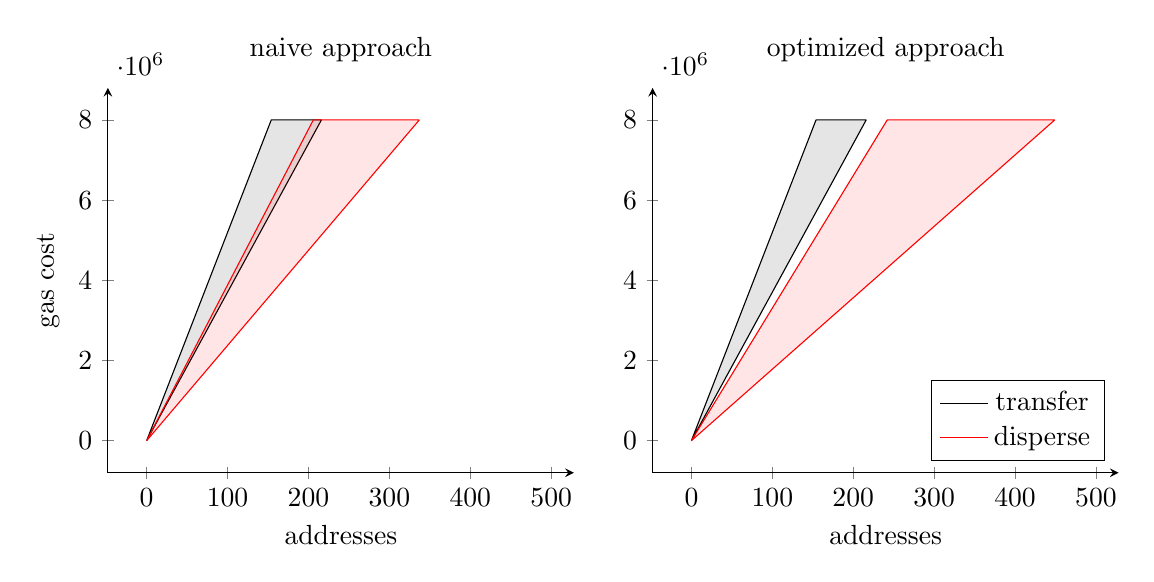
\begin{tikzpicture}
	\begin{groupplot}[
		width=7.5cm,
		xlabel=addresses,
		xmax=480,
		axis lines=left,
		enlargelimits,
		legend pos=south east,
		group style={
			group size=2 by 1
		}
	]
	\nextgroupplot[ylabel=gas cost, title=naive approach]
    \addplot[patch, black, faceted color=black, fill opacity=.1]
    coordinates {
        (0, 0)
        (154, 8000000) % token.transfer, 51947 gas, 30947 intrinsic
		(216, 8000000) % token.transfer, 36947 gas, 15947 intrinsic
    };
    \addplot[patch, red, faceted color=red, fill opacity=.1]
    coordinates {
        (0, 0)
		(206, 8000000) % token.transferFrom, 59400 gas, 38400 intrinsic
		(337, 8000000) % token.transferFrom, 44400 gas, 23400 intrinsic
    };
    \nextgroupplot[title=optimized approach]
    \addplot[forget plot, patch, black, faceted color=black, fill opacity=.1]
    coordinates {
        (0, 0)
        (154, 8000000) % token.transfer, 51947 gas, 30947 intrinsic
		(216, 8000000) % token.transfer, 36947 gas, 15947 intrinsic
    };
    \addplot[forget plot, patch, red, faceted color=red, fill opacity=.1]
    coordinates {
        (0, 0)
		(242, 8000000) % token.transferFrom, 59400 gas, 38400 intrinsic
		(449, 8000000) % token.transferFrom, 44400 gas, 23400 intrinsic
    };
    % for legend only
    \addplot[] coordinates {(0,0)};
    \addplot[red] coordinates {(100,0)};
    \legend{transfer, disperse}
	\end{groupplot}
\end{tikzpicture}
\caption{Comparison of naive and optimized approach}
\end{figure}


\subsection{Caveats}

ERC-20 interface dictates that all transfer functions should return \textit{true} on successful transfer.

However, there are at least 130 live tokens that don't follow this rule and return nothing.
The problem wasn't discovered for a long time because these tokens behaved as expected\cite{cremer}.
By pure coincidence the memory slot where the return value was expected contained the function selector which has always evaluated to \textit{true}.

Byzantium hard fork in November 2017 introduced a new RETURNDATASIZE opcode that allows for reading dynamically-sized data.
Contracts compiled with $solc \geq 0.4.22$ are checking the size of the returned data instead or blindly reading it from memory.
Such contracts won't be able to interact with these tokens.
Some of the more notable tokens affected are BNB and OMG.

The problem is fixable with inline assembly that handles both cases, but this fix is not a part of the contract presented for the sake of code simplicity.


\section{Further Optimization}

\subsection{Unlimited Allowance}
Allowance is oftentimes used as a binary switch.
A common pattern is to \textbf{approve} $\text{uint256}_{max}$ to grant unlimited allowance:

\begin{center}	
\begin{tabular}{r l}
	Allowance & Interpretation \\ \hline
	0 & disabled \\
	$2^{256}-1$ & enabled
\end{tabular}
\end{center}

There are at least two live ERC-20 tokens that utilize this pattern to optimize for gas usage.
0x protocol's own ZRX token interprets $2^{256}-1$ as a magic value meaning ``unlimited allowance" and skips updating the allowance on transfers in this case\cite{zrx-unlimited}. This allows to save 5000 gas on SSTORE and matches the cost of \textbf{transfer} and \textbf{transferFrom}.

Another example is Wrapped Ether (WETH), which is used to swap the native token to its ERC-20 form and back.

\subsection{Constantinople}

Constantinople is a code name for Ethereum hard fork which is set to go live in the beginning of 2019.
It is already live on Ropsten testnet at the time of publication.
Among other improvements, the fork changes the gas metering rules for SSTORE,
discussed in EIP-1283\cite{eip1283}.

The new gas costs and refunds are based on the combination of three values: original, current and new.
The logic became much more complex, but the gist is that the subsequent writes to the same storage slot during the transaction became much cheaper.

Consider the transitions of the contract token balance during an example transaction sending 1 token each to three recipients. The upper number shows the gas cost and the lower number shows the refund for clearing storage.
$$
0 \xrightarrow{20000} 3 \xrightarrow{5000} 2 \xrightarrow{5000} 1 \xrightarrow[-15000]{5000} 0 = 20000 \text{ gas}
$$
This is how it looks with EIP-1283 metering:
$$
0 \xrightarrow{20000} 3 \xrightarrow{200} 2 \xrightarrow{200} 1 \xrightarrow[-19800]{200} 0 = 800 \text{ gas}
$$

In generalized form with $n$ recipients:
$$G_{sset} + G_{sreset} \cdot n - R_{sclear} = 20000 + 5000 \cdot n - 15000$$
$$G_{sset} + G_{snoop} \cdot n - R_{sresetclear} = 20000 + 200 \cdot n - 19800$$

The total cost of updating the token balance for the contract is down from $5000 \cdot (n + 1)$ to $200 \cdot (n + 1)$ which is a 25x improvement.

Below is a comparison of how this change affects the performance of the proposed contract.


\begin{figure}[h]
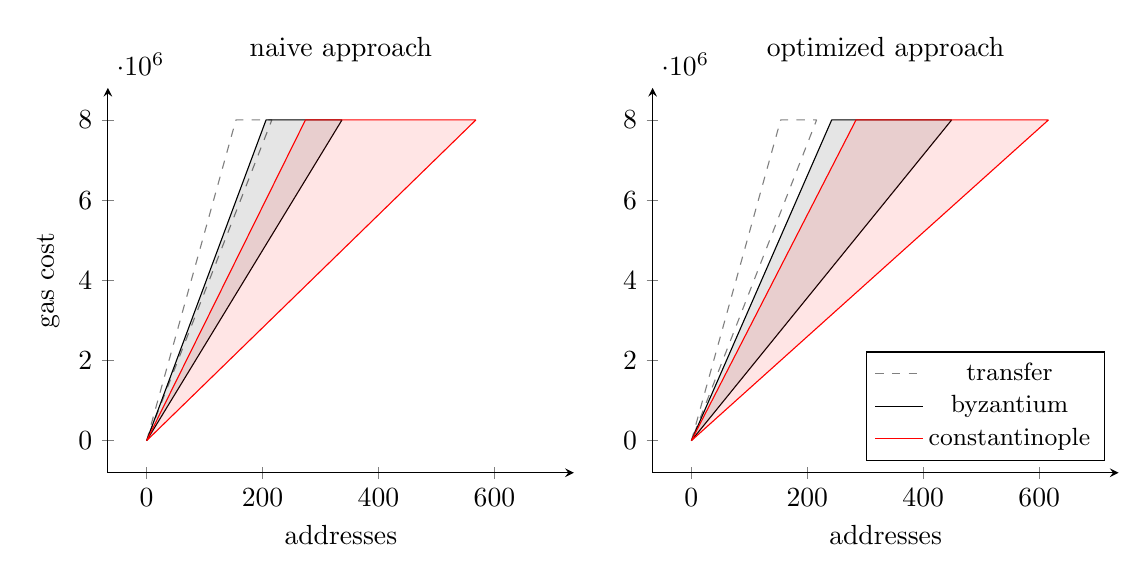
\begin{tikzpicture}
	\begin{groupplot}[
		width=7.5cm,
		xlabel=addresses,
		legend pos=south east,
		legend style={font=\small},
		xmax=670,
		axis lines=left,
		enlargelimits,
		group style={
			group size=2 by 1
		}
	]
	\nextgroupplot[ylabel=gas cost, title=naive approach]
	\addplot[forget plot, patch, dashed, faceted color=black!50, fill opacity=0]
    coordinates {
        (0, 0)
        (154, 8000000)
		(216, 8000000)
    };
    \addplot[forget plot, patch, black, faceted color=black, fill opacity=.1]
    coordinates {
        (0, 0)
        (206, 8000000)
		(337, 8000000)
    };
    \addplot[forget plot, patch, red, faceted color=red, fill opacity=.1]
    coordinates {
        (0, 0)
		(274, 8000000)
		(568, 8000000)
    };
    \nextgroupplot[title=optimized approach]
    \addplot[forget plot, patch, dashed, faceted color=black!50, fill opacity=0]
    coordinates {
        (0, 0)
        (154, 8000000)
		(216, 8000000)
    };
    \addplot[forget plot, patch, black, faceted color=black, fill opacity=.1]
    coordinates {
        (0, 0)
        (242, 8000000)
		(449, 8000000)
    };
    \addplot[forget plot, patch, red, faceted color=red, fill opacity=.1]
    coordinates {
        (0, 0)
		(284, 8000000)
		(616, 8000000)
    };
    % for legend only
    \addplot[black!50, dashed] coordinates {(0, 0)};
    \addplot[black] coordinates {(0, 0)};
    \addplot[red] coordinates {(0, 0)};
    \legend{transfer, byzantium, constantinople}
	\end{groupplot}
\end{tikzpicture}
\caption{Comparison of EIP-1283 effect on the algorithm}
\end{figure}

The overall effect is improvement from 242--449 transfers to 284--616 for optimized approach, which is a 1.17--1.37x better result and 1.84--2.85x improvement over non-batched transfers.


\section{Native Token}

{\color{red} write a chapter about sending ether}

\section{Methodology}

The gas usage is instrumented using Py-EVM\cite{pyevm}.
The benchmark setup is built from low-level primitives which include only the virtual machines with different rules and an in-memory state database. The mining and blockchain components were removed.

This allows to read and write directly to contract storage without the need to apply thousands of transactions to prepare for a test case.

Storage is accessed by index, in the same order as defined in the Solidity source\cite{read-storage}.
Mappings are accesses by keccak of their key and index, both of which are encoded as bytes32.
For example, balances mapping is accesses like this:
\begin{center}
	keccak(bytes32(address) + bytes32(0))	
\end{center}

Allowances can be accessed by repeating that twice:
\begin{center}
keccak(bytes32(spender) + keccak(bytes32(address) + bytes32(1)))	
\end{center}

All test cases use binary search to find the maximum number of transfers that can be fitted in a block.
The complete test suite \href{https://github.com/banteg/disperse-reseach}{can be found on Github}.

\section{Disperse}

The contract is deployed to Ethereum mainnet and all its testnets, as well as multiple other EVM-compatible networks:
\begin{quote}
	\href{https://etherscan.io/address/0xD152f549545093347A162Dce210e7293f1452150}{0xD152f549545093347A162Dce210e7293f1452150}
\end{quote}

There is also a client-only frontend interface hosted at \href{https://disperse.app/}{disperse.app}. It is built with riot.js and ethers.js.

\begin{thebibliography}{1}

\bibitem{ethereum} \href{https://www.ethereum.org}{Ethereum Project, 2015}
 
 \bibitem{eip20} \href{https://eips.ethereum.org/EIPS/eip-20}{Fabian Vogelsteller, Vitalik Buterin. {\em EIP 20: ERC-20 Token Standard}, 2015}

 \bibitem{openzeppelin} \href{https://github.com/OpenZeppelin/openzeppelin-solidity/blob/v2.0.0/contracts/token/ERC20/ERC20.sol#L151-L164}{OpenZeppelin-Solidity {\em Standard ERC20 token}, 2018}
 \bibitem{yellowpaper} \href{http://gavwood.com/paper.pdf}{Gavin Wood. {\em Ethereum: A Secure Decentralised Generalised Transaction Ledger}, Byzantium revision, 2017}
 	
 \bibitem{cremer} \href{https://medium.com/p/d67bf08521ca}{Lukas Cremer. {\em Missing return value bug--At least 130 tokens affected}, 2018}
 	
 \bibitem{eip1283} \href{https://eips.ethereum.org/EIPS/eip-1283}{Wei Tang. {\em EIP 1283: Net gas metering for SSTORE without dirty maps}, 2018}
 	
 \bibitem{multiplexer} \href{https://github.com/DigixGlobal/multiplexer}{DigixGlobal. {\em Multiplexer}, 2017}
 	
 \bibitem{solidity-errors} \href{https://solidity.readthedocs.io/en/latest/control-structures.html#error-handling-assert-require-revert-and-exceptions}{Solidity Documentation. {\em Error handling in Solidity}, 2018}
 	
 \bibitem{zrx-unlimited} \href{https://github.com/0xProject/0x-monorepo/blob/48ff13e3e22bf9f71bc1a367f86aaa0ae89989ae/packages/contracts/contracts/tokens/ZRXToken/UnlimitedAllowanceToken_v1.sol#L43-L45}{0x Project. {\em Unlimited Allowance Token v1}, 2017}
 
\bibitem{pyevm} \href{https://github.com/ethereum/py-evm}{Py-EVM. {\em A Python implementation of the Ethereum Virtual Machine}, 2018}

\bibitem{read-storage} \href{https://medium.com/aigang-network/how-to-read-ethereum-contract-storage-44252c8af925}{Darius. {\em How to read Ethereum contract storage}, 2017}

\end{thebibliography}

\appendix


\section{Summary Tables}

Here is a summary table of different strategies outlined in this paper. All numbers assume a transaction filling the whole block gas limit.

\begin{table}[h]
	\caption{Gas usage per token transfer}
	\begin{center}
	\begin{tabular}{l r r}
		Function & Byzantium & Constantinople \\ \hline
		transfer & 36,947--51,947 & 36,947--51,947 \\
		transferFrom & 44,400--59,400 & 44,400--59,400 \\
		naive & 23,694--38,739 & 14,082--29,145 \\
		optimized & 17,813--32,928 & 12,977--28,092 \\	
	\end{tabular}
	\end{center}
\end{table}
%
\begin{table}[h]
	\caption{Max token transfers per block}
	\begin{center}
	\begin{tabular}{l r r}
		Function & Byzantium & Constantinople \\ \hline
		transfer & 154--216 & 154--216 \\
		transferFrom & 134--180 & 134--180 \\
		naive & 206--337 & 274--568 \\
		optimized & 242--449 & 284--616 \\	
	\end{tabular}
	\end{center}
\end{table}


\end{document}
